%======================================================================
\chapter{API Usage Patterns Study}
\label{sec:apiusage}
%======================================================================
We aim to take a snapshot of where current software practices stand: we investigate how APIs are used and misused. Our goal is to investigate API usage patterns, both conceptually and in practice.
Such patterns can provide interesting hints for API designers in the future.

We begin by defining two terms that we use in this work, followed by an example. 
A library's \emph{intended API surface} is the set of
classes, methods and fields that it expects clients to use. Other
classes, methods and fields are \emph{internal} to the library. Using
internal parts of the library involves some sort of \emph{bypass}. On
the other hand, a client uses an \emph{actual API surface} of the
library. In the absence of bypasses, the actual surface is a subset of
the declared surface.


\begin{figure}[h]
 \begin{center}
  \begin{tikzpicture}
    \node (client-a) at (3.3, 0.5) {$u_a$};
    \node (client-b) at (3, 1.7) {$u_b$};

    \node (class-1) at (-1.5, -1.3) {\texttt{C}$_1$};
    \node (class-2) at (1.7, -1.2) {\texttt{C}$_2$};
    \node (class-3) at (1.5, 1) {\texttt{C}$_3$};
    \node (class-4) at (-1.5, 1) {\texttt{C}$_4$};
    \node[draw] (class-5) at (0,0) {\texttt{C}$_5$ (internal)};

    \draw (-2.1, -1.6) rectangle (2.1, 1.5);

    \node (lib) at (-1.4, 1.7) {Library $L$};

    \draw[-Latex] (client-a) -- (class-2);
    \draw[-Latex] (client-a) -- (class-3);

    \draw[-Latex] (client-b) -- (class-3);
    \draw[-Latex] (client-b) -- (class-4);
  \end{tikzpicture}
  \caption{API surface of library $L$, which exports classes \texttt{C}$_1$ through \texttt{C}$_4$. Class \texttt{C}$_5$ is internal and direct calls to it are not allowed. Client $u_a$ uses classes \texttt{C}$_3$ and \texttt{C}$_2$, while client $u_b$ uses classes \texttt{C}$_4$ and \texttt{C}$_3$.}
  \label{fig:api-surface}
 \end{center}
\end{figure}


Figure~\ref{fig:api-surface} illustrates the situation where library
$L$ is used by clients (users) $u_a$ and $u_b$. $L$'s intended API surface
includes classes \texttt{C}$_1$ through \texttt{C}$_4$, while class
\texttt{C}$_5$ is internal to $L$, and uses of it involve bypasses. We
have evidence that the actual API surface includes classes
\texttt{C}$_2$ through \texttt{C}$_4$, and we don't know about whether
\texttt{C}$_1$ is used by any extant client.


\section{Methodology}
\label{sec:methodology}

We now describe the implementation of our tool and our benchmark selection process.

\subsection{Static Analysis and Instrumentation}
\label{sec:methodology}

We use Javassist~\cite{chiba00:_load_struc_reflec_java} and perform class hierarchy analysis on clients
and create a static call graph. We collect data about client usages of libraries by running client
test suites under instrumentation. The instrumentation records API
uses which cross client/library boundaries, closely mirroring the API
usage patterns that we describe in
Section~\ref{sec:patterns}. We also use Javassist for instrumentation,
and the build system of each project (Maven) is used to run its
tests and we obtain dynamic call graphs. 
\\

\begin{figure*}[h]
 \begin{center}
\resizebox{0.9\textwidth}{!}{
  \begin{tikzpicture}
    \node[block] (client) {client};
    \node[block,below=1cm of client] (library) {library};

    \draw (library) -- node[left] (depends) {depends on} (client);

    \node[above left=.75em of client] (ja) {\begin{minipage}{7em} modify \\with Javassist \end{minipage}};
    \draw[-Latex] (ja) -> (client);
    \draw[-Latex] (ja) to [->,bend right=35] (library.west);

    \node[block, above right=2em of client,xshift=-2em] (olib) {other library};
    \draw (client) -- node[right,xshift=.1em] (also) {also depends on} (olib);

    \node[oval,right=of depends] (test) {maven/gradle: run tests};

    \draw[-Latex] (client) to [->,bend left=15] (test);

    \node[block, right=10em of client] (output) {test output};
    \node[block, right=10em of library] (raw) {raw API usage info};

    \draw[-Latex] (test) to (output);
    \draw[-Latex] (test) to (raw);

    \node[oval, right=of raw] (Py) {Python scripts};
    \draw[-Latex] (raw) to (Py);

    \node[block, right=1em of Py] (viz) {D3 visualizations};
    \draw[-Latex] (Py) to (viz);
  \end{tikzpicture}
}
  \caption{Our instrumentation workflow. Using Javassist, we analyze and instrument clients and run their test suites. (We process the generated data with Python scripts to create D3 visualizations for VizAPI.)}
  \label{fig:workflow}
 \end{center}
\end{figure*}

Figure~\ref{fig:workflow} summarizes our instrumentation and
data capture workflow. We next describe our instrumentation implementation in detail.

We identify interactions across the client/library boundaries by inspecting JAR files of
each software component to obtain a list of classes for every component. We associate classes 
and their members to components based on these lists. Since the JAR files contain source code,
we ensure that none of the library uses meant solely for unit testing are captured.

\paragraph{Vanilla invocations}
The standard case is simple. At every invoke instruction in every
loaded method which transfers control between the client and the
library, we add code to record that invoke by incrementing a counter.
We handle both static and virtual (including special, virtual,
interface, and dynamic) calls. Crossing the client/library boundary
includes conventional calls from the client to the library as well as callbacks from the library to the client.  

\paragraph{Field accesses}
We capture direct (field sets and gets) and reflective (via invocations of
\texttt{java.lang.reflect.Field.get()} and \texttt{.set()}) field
accesses.

\paragraph{Dynamic proxies and reflective calls}
We specially handle invocations of the distinguished method 
\texttt{java.lang.reflect.Method.invoke()} method used to invoke dynamic proxies and reflective calls, recording
details of the calls that we intercept. 
We identify dynamic proxies by checking whether the invocation 
of \texttt{Method.invoke()} originates from a class that implements 
\texttt{java.lang.reflect.InvocationHandler}. If so,
we inspect the call stack to find the caller and callee of 
\texttt{Method.invoke()} and record the call if it crosses the client/library boundary. 
All other calls to \texttt{Method.invoke()} are standard reflective calls, 
and we record the respective callers and callees.
(We also specifically ignore calls to \texttt{Method.invoke()} made by the Maven surefire plugin
as it runs tests.)
% \todo[inline]{When running tests, the Maven surefire plugin uses the invoke method too,
% which is ignored. Should we talk about that?}

Instrumenting methods also allows us to capture several other library uses,
as we describe below.

\paragraph{Class usages}
We capture reflective uses of the \texttt{Class} object by intercepting calls to
\texttt{java.lang.Class.forName()} and \texttt{java.lang.ClassLoader.loadClass()}.

\paragraph{Service Loaders} We are particularly interested in bypasses of 
services using \texttt{ServiceLoader}. Before the instrumentation, we record a list 
of services and their implementations by inspecting files in \texttt{src/main/resources/META-INF/services}.
With this information, we look for service bypasses which are direct uses of service implementation 
classes in clients either through instantiations, casts or reflection. We also intercept calls 
to method \texttt{load()} in classes with name \texttt{Service*Loader} and record any calls to methods beyond 
the published interface.

\paragraph{setAccessible()} 
Java provides the \texttt{setAccessible()} method to allow reflective access to class members despite
access modifiers. After a call to this method, the program may then (subject to security manager restrictions)
reflectively access the class member.
We thus record calls to \texttt{setAccessible()} along with the previous visibility of the class member.

\paragraph{Annotations} 
We have a quasi-static approach for finding class, field and method
annotations: we observe all annotations for a class or class member
when it is loaded, and record cases where a class or member declares an
annotation from the library of interest. We also record an association
between the class and its memers' annotations.

\paragraph{Inheritance and interface implementation} At load time,
we also record information about all superclasses and implemented interfaces
that cross the library/client barrier.

\paragraph{Instantiations and casts} We also instrument the
\texttt{NewExpr} and \texttt{Cast} bytecodes to record library/client 
instantiations and casts.



\subsection{Benchmark Selection}
\label{sec:benchmark}
Our benchmark set consists of 11 libraries and 90 clients. For libraries, we pick the most popular Maven 
repositories in different categories such as logging, json parsing and databases. Table~\ref{tab:libs} presents our set of libraries. We measured lines of code (kLOC) using SLOCcount\footnote{\url{https://dwheeler.com/sloccount/}} and number of classes by building libraries and counting resulting \texttt{.class}es. A project uses ServiceLoaders if it has a \texttt{META-INF/services} directory and Java 9 modules if it has a \texttt{module-info.java} file. A library is an OSGi component if it contains a \texttt{MANIFEST.MF} file in its build output\footnote{Some libraries (e.g. \emph{connector-j}) create OSGi metadata during the build, so we look for the metadata in the output, not in the source.}, and this manifest contains \texttt{Export-Package} declarations. 

\begin{table*}[ht]
\begin{center}
\caption{\label{tab:libs}Libraries that we investigated for API usage and mis-usage patterns}
\begingroup\scriptsize	
\hskip-2.0cm
\begin{tabular}{l!{\color{verylightgray}\vrule}cl!{\color{verylightgray}\vrule}rr!{\color{verylightgray}\vrule}ccc}
& & & non-test &  & Service & Java 9 &  \\
Library & version & description   & kLOC     & \# classes  &  Loader  & modules & OSGi \\ \arrayrulecolor{verylightgray}\hline
commons-collections4 & 4.4 & data structure implementations & 28.9 & 524 &&&\checkmark\\
commons-io & 2.8.0 & IO functionality library & 12.6 & 182& & &\checkmark\\
joda-time & 2.10.10 & date and time handling library & 28.9 & 247&&& \checkmark \\
slf4j-api & 1.7.9 & logging library & 1.5 & 28 & & & \checkmark\\
jsoup & 1.13.1 & HTML parser & 12.5 & 249&&&\checkmark\\
fastjson & 1.2.76 & json parser/generator & 43.6 & 260 &\checkmark&\\ 
gson & 2.8.8 & json parser/generator & 14.4&  182 && \checkmark&\checkmark\\
json & 20210307 & json parser/generator & 11.8 & 27& & \\
jackson-core & 2.12.3 & json parser/generator & 27.1 & 124 & \checkmark&  \checkmark&\\
jackson-databind & 2.12.3 & bindings for json parser/generator & 68.2 & 700 & \checkmark & \checkmark&\\ 
h2 & 1.4.200 & database & 147.2 & 1010 & \checkmark & & \checkmark \\
\end{tabular}
\endgroup
\end{center}
\end{table*}

We use the libraries.io dataset\footnote{\url{https://libraries.io/}}, to construct a dependency graph and look for the most used upstream components (highest number of other components depends on [any version of] those), 
and the top downstream components (clients). We exclude any clients that have less than 10 stars or less than 10 forks on Github.  Apart from this, we also pick a subset of projects from the
Duets benchmarks~\cite{durieux21}. We exclude components that do not contain unit tests, components that use our chosen library only for testing
and components that declare the library as a dependency in their POM file, but do not actually use it. Our benchmark set contains both Maven single module and multi-module components.

We executed each of the clients' test suites to collect data about how the clients use all of their dependencies; our data therefore includes not just interactions between our clients and the 11 libraries sampled, but also ``bycatch''---that is, other libraries that are also called by the clients (``also depends on'' in Figure~\ref{fig:workflow}) and the libraries. The total static transitive closure of dependencies of our clients includes 4297 components.

Collecting execution data from programs is more challenging than it seems: downloading software and collecting static numbers is fairly straightforward, but running this software to instrument it involves fixing numerous uninteresting environment glitches which nevertheless block progress---even in the stable environment of a continuous integration system at a large software company, Kerzazi et al~\cite{kerzazi14:_why_do_autom_build_break} found that 17.9\% of builds break, and our context is even more challenging.

We have made our data publicly available\footnote{\url{https://zenodo.org/record/6951140}}.


\section{Classification of API Uses}
\label{sec:classification}

We now present a conceptual framework that outlines four dimensions along which a potential API use can be classified. We phrase the four dimensions as questions; each API usage has an answer for each of the questions. They are as follows: \emph{what}, \emph{how} \emph{which way} and \emph{why not}?

\begin{enumerate}
\item \emph{What} thing is being accessed?
\begin{itemize}
    \item types: user declares a subtype of a provider type;
    \item classes: user instantiates an object of a provider's class;
    \item annotations: user annotates a class or member with a provider-defined annotation;
    \item methods: user invokes a method from the provider; and,
    \item fields: user accesses a field defined in the provider.
\end{itemize}
\item \emph{How} is it accessed?
\begin{itemize}
    \item direct: user directly names thing being accessed;
    \item indirect: (methods only) thing being accessed differs from thing on declared type of the receiver object;
% we are using a runtime definition of virtual here: even if the call is declared virtual, we're calling it direct if declared target = actual target
    \item reflection/unsafe: user creates a handle to thing being accessed and uses that handle to perform the access;
% Mastrangelo says that, for our context, unsafe is used for serialization/deserialization, as sort of a super reflection.
    \item advanced dynamic: none of the above---user accesses thing in some other way, e.g. via proxies.% or runtime code generation.
\end{itemize}
\item \emph{Which way} is the access going?
\begin{itemize}
    \item client user to library provider;
    \item library user to client provider, via callbacks.
\end{itemize}
\item \emph{Why not}, i.e. is the user bypassing access control?
\begin{itemize}
    \item access modifiers prevent the access, but are overridden;
    \item modularity conventions or mechanisms prevent the access: ``internal'' package, Java 9 modules, or OSGi;
    \item service loader restrictions prevent the access.
\end{itemize}
\end{enumerate}

The ``why not'' dimension differentiates uses from misuses; an API use that is allowed and expected by the API developer does not have an answer for ``why not''. Considering intended versus actual API surfaces gives another
perspective on the ``why not'' question. The other dimensions serve to classify the API use or misuse and understand which kinds of uses and misuses are most common. We intend for this framework to serve as a guideline for component developers who want to introspect about their software. Library developers can use this framework when they design new APIs to understand which parts of their library are most useful to clients and how. Client developers can use this framework to inspect how libraries are used and possibly to compare and contrast different libraries with the same functionality.

We suggest that it is useful to think of misuse as on a
continuum rather than as a strict binary allowed-versus-not-allowed.
Some uses are more appropriate than others: when a
client passes an object to a serialization library, it is asking
the library to access even the private fields of that object, and so this
does not constitute a mis-use. Calling a deprecated API is less clear-cut.
Finally, explicitly calling into internal classes is likely to be a mis-use.
All bypasses some incur technical debt and add to the project's risk,
but some bypasses are more risky than others.


\section{API Usage Patterns}
\label{sec:patterns}

We now discuss API usage patterns with examples. Our examples use the \textit{connector-j} library\footnote{\url{https://github.com/mysql/mysql-connector-j/}, release 8.0.26}, which enables Java programs to communicate with MySQL databases. Namespaces are omitted for brevity. The standard Java library JDBC types belong to package \texttt{java.sql} and MySQL classes to packages \texttt{com.mysql.cj.jdbc.*}. Most of the code snippets are not considered best practice, and therefore illustrate API misuses.


\subsection{Vanilla API Usage}

\lstdefinestyle{mystyle}{
	basicstyle=\ttfamily\footnotesize,
	breakatwhitespace=false,         
	breaklines=true,                 
	captionpos=b,                    
	keepspaces=true,                 
	numbers=left,                    
	numbersep=5pt,                  
	showspaces=false,                
	showstringspaces=false,
	showtabs=false,                  
	tabsize=2,
	frame = single
}

\lstset{style=mystyle}


MySQL JDBC driver class \texttt{com.mysql.cj.jdbc.Driver} implements the \texttt{java.\-sql.\-Driver} interface from the standard Java library. This is a case where the user, \textit{connector-j}, is a client of the standard library API. It is not bypassing any access control, directly accessing a \emph{type} from its library, and the access is going from the client to the library.

Shifting perspectives, \textit{connector-j} is intended for use as a library by its own clients. Its \texttt{Driver} implementation has a public constructor that can be \textit{directly instantiated} by its clients, as shown in line 1 of Listing~\ref{listing:direct-invocation}. It turns out that clients are not supposed to instantiate \texttt{Driver} classes themselves---JDBC documentation states that, for recent versions of JDBC, clients are supposed to call \texttt{DriverManager.getConnection()}. However, there are no compile-time or run-time checks prohibiting the instantiation of this object. We call this a \emph{modularity convention violation}. The part of the library that is being accessed is a class and the access is going from client (shown) to library (\texttt{connector-j}).  Although direct instantiation is not the intended use of the API, the library must provide a public constructor to enable service discovery.

Continuing with our example, line 2 of the same Listing~\ref{listing:direct-invocation} shows a \textit{direct invocation}. Although this call is a virtual method invoke, the declared type and actual types will always coincide in this example. There is no access control bypass here, and this is a direct invocation of a method call from the client to the library. We also observe \emph{indirect invocations}, i.e. virtual invokes where declared and actual differ.

%% In OO code, declared and actual types often differ, as seen at line 2 of Listing~\ref{listing:indirect-invocation}). The declared type is the interface \texttt{java.sql.Driver} while the actual type is class \texttt{com.mysql.cj.jdbc.Driver}. The only change between this \emph{indirect invocation} and the previous call is that the access is indirect, not direct. 

%The Java Virtual machine also includes the invokedynamic instruction to allow programmable method dispatch. The Java compiler occasionally generates this instruction, e.g. for dynamic code idioms like lambdas. There is no explicit receiver object for an invokedynamic and we do not consider such calls.

\lstinputlisting[language=Java,caption=Direct Instantiation and Invocation,label=listing:direct-invocation]{code-snippets/direct-invocation.java}

%% \lstinputlisting[language=Java,caption=Indirect Invocation,label=listing:indirect-invocation]{code-snippets/direct-virtual-invocation.java}

Our classification also allows for direct field accesses---from client to library or vice-versa (in the library to a client-provided parameter object). Of course, these may come with or without access control bypasses.

\subsection{Reflection and Reflective API Bypasses}
\label{ssec:api-usage-patterns:api-bypass}
Java reflection provides an alternate way for users to access APIs, i.e. it is an alternate ``how" something is accessed. Reflective accesses exist in practice and are more challenging to analyze statically than vanilla usages, as investigated by Landman et al~\cite{landman17:_chall_static_analy_java_reflec}; however, Bodden et al~\cite{bodden2011taming} have presented pragmatic workarounds based on recording dynamic information and using it statically. Clients request a reflective handle to classes, methods (and constructors), and fields, and call certain Java API methods to access the thing behind the handle. Listing~\ref{listing:reflection} shows a reflective instantiation of a \texttt{Driver}; prior to JDBC 4, this used to be the recommended way of creating a JDBC driver, but has been superceded by using a \texttt{DriverManager} to get a connection. We understand that this is not explicitly forbidden, but it is deprecated.

%% Instantiation, method invocation and field access is also possible through the reflection protocol in standard classes \texttt{Class}, \texttt{Method}, \texttt{Constructor} and \texttt{Field} in\texttt{ java.lang} and \texttt{java.lang.reflect}, respectively. We refer to these categories as \textit{INST-R}. \textit{INV-R }and \textit{FACC-R}, respectively. An example for reflective instantiation is shown in 

\lstinputlisting[language=Java,caption={Instantiating a \texttt{java.sql.Driver} via reflection},label=listing:reflection]{code-snippets/reflection.java}

Even if constructors, methods and fields and the classes declaring them are not visible, reflection can still be used to instantiate, invoke or access the respective things, subject to permission being granted by security managers. Listing~\ref{listing:reflection-private} shows the use of reflection to bypass access modifiers. While the class \texttt{ConnectionImpl} is public, the no-argument constructor has access modifier \texttt{protected}. However, reflection allows users to override access restrictions and call that constructor anyway. These are examples of a \textit{reflective API bypass pattern}. This call is thus a reflective-API-bypassing access to a constructor via reflection, from the client to the library. Line 3 makes the constructor accessible, using a pattern known as ``deep reflection''. Under Java 9, a user must provide a specific parameter to the JVM to allow such calls.

Java has mechanisms for preventing unwanted reflective accesses in general. In addition to preventing deep reflection and providing security managers, Java 9 also displays warnings about illegal reflective accesses to JDK internals. (Reflection can, of course, also be used to make calls that are part of a library's published API.)

\lstinputlisting[language=Java,caption=''Deep reflective'' instantiation bypassing visibility constraints,label=listing:reflection-private]{code-snippets/reflection-private.java}

% interesting but maybe not our point; I said things about it above.
%% Interestingly, prior to JDBC4, reflection was used to install a driver, consisting of the \texttt{Class.forName} call shown in line 1 of Listing~\ref{listing:reflection}. This triggered the execution of the static block of the respective class, leading to the instantiation and registration of the driver in  the JDBC  registry. 

%\todo[inline]{java 9 has illegal-reflective-access warnings which protects JDK internals from reflection. also they call it ``deep reflection'' when you use setAccessible to access private members. --add-opens allows this in java 9}

At this stage, we'd like to reiterate our goal in investigating API accesses. We've discussed vanilla API usages and reflective accesses to APIs. These two types of accesses have different affordances in terms of program evolution, and we aim to empirically evaluate how developers access libraries in practice, so that we (and others) can develop tools to help developers achieve more stability.

Upon a breaking upgrade, a vanilla API usage will fail to compile. Reflection is more dynamic---developers have the power to query the system and to adapt to the actual versions of the components that they are interacting with. If they use this power, then their code can be more resilient. However, failures that do arise can be more subtle and severe. The same phenomenon is present in Rinard's acceptability-oriented computing~\cite{rinard03:_accep}.

Dynamic techniques like reflection in data binding and persistence mapping pose additional perils. Even minor changes to classes can render data produced with previous versions un-readable. Adding, removing or modifying a field in a class mapped to a relational database table requires altering the table and migrating data. Adding a custom constructor (and thereby removing the default constructor) or removing a setter method may derail a deserialization mechanism based on the Java bean model (e.g. \texttt{java.bean.XMLDecoder}). Binary serialization has long suffered from this problem. 

\subsection{Restricting API surfaces: Services, Package Names and Package Exports}
We mentioned that reflective instantiations of \texttt{Driver}s were recommended prior to JDBC 4. Post-JDBC 4, the recommendation is now to use the service loading mechanism to further reduce dependencies of clients on particular drivers. Specifically, the client is to use the \texttt{DriverManager} abstraction, which allows multiple drivers to bid on establishing a connection for a given database URL. (The client does not use the service loader directly.) 

\lstinputlisting[language=Java,caption={\tt Driver} instantiation through a service loader,label=listing:service-loader]{code-snippets/service-loader.java}

Service loading (described by Fowler in~\cite{fowler04:_inver_contr_contain_depen_injec}) is now widely used to register and access service implementations, e.g. parsers, character sets, JDBC drivers, and JUnit5 extensions. 
Listing~\ref{listing:service-loader} shows an example of a client requesting an available \texttt{Driver} from a service loader (and not the {\tt DriverManager}) and using that driver to request a jdbc MySQL connection.
%Similar features for declarative services have been available for some time as part of OSGi~\footnote{OSGi services provide more features than Java service loading, including e.g. lifecycle management for services and the ability to wire, un- and rewire clients to the services they consume, but these are not relevant here.}. 

%Libraries advertise services as part of their metadata. This advertises both the capabilities of a component and its intended API. [Do we need this?]

Access modifiers are not the only way to protect APIs from being
called directly by clients.  Java's namespace is segregated by
hierarchical package names, but there are no enforced access controls
in plain Java. The Java standard library does state the modularity convention
that some of its implementation (specifically the classes living in
the \texttt{sun.*} namespace) is not to be used by clients, but this
convention is not enforced. Many libraries also use the convention that packages
named \texttt{internal} are not for use by clients. 

Java 
9 modules~\cite{corporation17:_java_platf_modul_system_jsr} and OSGi~\cite{alliance20:_osgi_core_releas_specif} offer other ways to delimit an intended API, in terms of a set of exported
packages. However, without enforcement, clients can use
all of the methods and fields of their libraries.

Enforcing the stated constraints requires additional support---either
a Java 9+ runtime or an OSGi container implementation. The Java 9+
compiler and runtime ensure that modules do not access modules to
which they do not have access, e.g. non-exported modules. Under Java
9+, modules can also rely on having fine-grained control over
reflection permissions. Similarly, under an OSGi container implementation,
non-exported packages are invisible to other code in the same Java
Virtual Machine, and this is enforced using the class loader
mechanism. 

We run all of our clients and libraries unprotected by Java 9 modules
and OSGi containers---this is an opportunity to observe whether developers
bypass the stated constraints or not. As we'll see in Section~\ref{sec:results}, 
they almost universally do not bypass constraints.

%% However, to enforce this (i.e. that clients only used API in those packages) requires a runtime to support this, i.e. an OSGi container (for components complying to OSGi, also known as \textit{bundles}), or a Java 9+ runtime. 

%% In case of connector-j, OSGi meta data is created during the build, the respective exported packages are defined in the ANT build script  \texttt{build.xml}. 


%% \todo[inline]{Do we have cases of library/client interactions via OSGi (as opposed
%% to via declaring as a plain old Maven/Gradle dependency and making a
%% normal method invoke?) If a client was using a library through OSGi
%% then it wouldn't be able to violate the do-not-call restrictions, but
%% it could cast a type to see more method implementations than it should
%% be able to.} Actually I don't think that you can do the downcast trick with OSGi
%% because you can't see the thing that you'd like to downcast to.

By advertising services or exported packages, components define an intended API. Clients should not have any additional compile-time dependencies on the component beyond the intended API: any such additional dependencies become API bypasses. In particular, any of the following is an API bypass if it occurs in client code: 

\begin{enumerate}
	\item instantiation of a type declared in the component but not defined in the intended API;
	\item reference to a type declared in the component (\texttt{T.class}; casts \texttt{(T)}; or uses of annotation types) not defined in the intended API;
	\item invocations of method implementations which are not part of the intended APIs, following a downcast from an intended API to a private API; or,
	\item accesses to fields not defined in the intended API.
\end{enumerate}
% declared in the components other then virtual calls of methods not declared in the component are resolved to methods declared in the component


\subsection{Reversing Directions: Callbacks and Dependency Injection}
We think of clients calling libraries. However, callbacks from libraries to clients are common in practice: the client provides an object to the library, and then library calls back a pre-defined method on the client. Callbacks are especially ubiquitous in languages like JavaScript, but do occur in Java code. Fowler~\cite{fowler05:_inver} uses the term ``framework'' to describe callback-heavy libraries that practice this Inversion of Control.
% Many callbacks are based on the Observer pattern. - I don't think we need to say that.

%While method invocations that are part of component interactions generally consist of clients invoking methods provided by some other component, this direction can be reversed when clients pass references to objects to be used in virtual calls. This popular pattern is based on the observer pattern, and often referred to as callbacks. It is particular popular in languages like JavaScript. 

JDBC uses callbacks to tell its clients about events that happen to connections, as shown in Listing~\ref{listing:callback}. Call sites for callbacks live in the library \textit{connector-j}, and the respective invocations are virtual calls in JDBC resolved at runtime to invocations of methods that live in the client.

\lstinputlisting[language=Java,caption=Callbacks in JDBC,label=listing:callback]{code-snippets/callback.java}

Callbacks can be reflective. This is widely used in JSON and XML data binding and object-relational mapping. For instance, the \textit{jackson} object mapper and the XML serializer in the Java standard library can serialize instances of Java classes by exploiting reflection and Java Bean programming patterns. That is, the library accesses non-public fields in the client by discovering getters and invoking them dynamically, rather than reflectively reading the fields. Note the direction of the access---from library to client. This is an example of an API bypass that is not a mis-use.
% it looks really ugly.
%~\footnote{In jackson, this is implemented in \texttt{com.fasterxml.jackson.databind.ser.BeanPropertyWriter::serializeAsField}}. 
%This creates reflective callbacks from an upstream component into a client.

%\todo[inline]{Hey! From the writing here jackson and guava both access non-public fields, i.e. no difference. Is that true? -> jackson uses getters and setters, guava doesn't.}

A popular alternative to \textit{jackson} is \textit{guava}. That library instead directly accesses even non-public fields, bypassing access restrictions\footnote{See \texttt{UnsafeReflectionAccessor::makeAccessible} in package \texttt{com.google.gson.internal.reflect}.}, as discussed in Section~\ref{ssec:api-usage-patterns:api-bypass}. Note that the general idea of reversing the direction of API access is not restricted to method calls but also extends to fields.

\subsection{Beyond Reflection}

There are several other techniques that allow dynamically using code provided by libraries. Dynamic proxies (\texttt{java.lang.reflect.Proxy}) can be used to dynamically subtype existing types, with invocation handlers being used to provide any required method implementations.  This mimics protocols like Smalltalk's \texttt{doesNotUnderstand}, and was originally used to provide stubs for remote object protocols like RMI and CORBA, and later in some mock object frameworks. However, usage is rather rare~\cite{dietrich2017xcorpus}, and modern remoting and mock testing frameworks (in particular, protocol buffers and mockito) use some form of code generation instead. 

An older dynamic mechanism is the \texttt{sun.misc.Unsafe} API. Mastrangelo et al~\cite{mastrangelo15:_use_your_own_risk} pointed out that Java's undocumented 
\texttt{Unsafe} API was extensively used in practice to circumvent the safety properties guaranteed by the Java Virtual Machine. Since then, this API has been migrated to a \texttt{jdk.unsupported} module, and Evans~\cite{evans20:_unsaf} noted that many of the features have been  migrated into supported Java APIs.

The \texttt{invokedynamic} instruction can also be used as an intermediate mechanism to access APIs via custom dispatch. However, the usage patterns defined by the current Java compiler restrict the use to the compilation of lambdas and string concatenation only.  There might be more interesting API access patterns in clients compiled with non-Java compilers (such as Kotlin), but this is outside the scope of this study. 


%\todo[inline]{I don't actually think dynamic proxies are very interesting in terms of API bypasses, but I think that unsafe is good to talk about here.}

%Several advanced techniques are available to as alternatives to reflection. This is driven either by performance consideration, or by the need to create functinality at runtime (instead of just querying the object model). A typical use case here is to replace an interpreter by a more performant compiler for some domain specific language. 



%\todo[inline] { Jens $\rightarrow$ Pat: can we move this to related work, it does not fit well into the story here
%For our purposes, Mastrangelo et al observed two potentially relevant\texttt{Unsafe} usage patterns: (1) serialization/deserialization, and (2) load class without security checks.  Serialization is ubiquitous, being transitively used in 5689 of 21287 artifacts. Loading without security checks was much less common, transitively used in 294 of 21287 artifacts. A third pattern is extremely common but, we claim, unlikely to lead to modularity violations---allocating objects without calling their constructors, used in mocking and deserialization. }

%\todo[inline] { Jens $\rightarrow$ Pat: I would not mention modularity here because we dont really discuss this, instead we should state whether it can violate API access restrctions In principle, \texttt{Unsafe} or its newer equivalents could be used to violate modularity. However, we believe that the patterns observed in practice are unlikely to correspond to actual violations. }

In principle, \texttt{Unsafe} or its newer equivalents could be used to bypass API restrictions. However, we believe that the patterns observed in practice are unlikely to correspond to actual bypasses.

% OK, so dynamic code generation could be a thing that matters sometimes, but not often enough that we want to talk about it here.

% However, modern mock object frameworks like Mockito often use the on-the-fly generation of  classes. This is facilitaed by the availability of modern bytecode engineering libraries like ByteBuddy\footnote{\url{https://bytebuddy.net/}} that make it very easy to create and load classes at runtime. Other examples for using runtime code generation include high-performance expression engines (MVEL), and the Xalan XSLT cmpiler creating the aptly named GregorSamsa classes~\footnote{\url{https://xml.apache.org/xalan-j/xsltc/xsltc_native_api.html}}. 

% \todo[inline]{I think we don't quite have alignment on what we're trying to say here. I think that Unsafe fits here while on-the-fly generation of classes doesn't.}

% \todo[inline] {Jens: should we also at least mention invokedynamic here ? Not an issue with the Java compiler, but perhaps for oother JVM languages. PL: I don't see how it's particularly relevant here. It's just a method call. At best it's another alternative for ``how'' is it accessed, but really it is just indirect.}


\section{Results}
\label{sec:results}

We look for our usage patterns in our benchmark collection of 11 libraries (Table~\ref{tab:libs}).

\subsection{API bypasses}
We first investigate the use of API bypasses in our clients. This is useful to library developers if they want to identify which parts of their libraries that are supposed to be internal are actually used by clients. This can help them with API design in future versions. In Section~\ref{sec:classification}, we enumerated three broad categories
of bypasses: access modifiers, modularity conventions, and service loaders. We discuss each of them in turn.


\paragraph{Access modifiers and reflection}
% latex table generated in R 4.2.0 by xtable 1.8-4 package
% Tue Aug 23 13:16:06 2022
\begin{table}[ht]
\centering
\begingroup\small
\begin{tabular}{llllr}
  \hline
Library & Client & Member & Visibility & Count \\ 
  \hline
libthrift & benchmark-thrift & Field & private & 1 \\ 
  spring-context & fastjson & Constructor & private & 1 \\ 
  javax.servlet-api & fastjson & Field & private & 9 \\ 
  spring-context & fastjson & Field & private & 22 \\ 
  javax.servlet-api & fastjson & Method & public & 17 \\ 
  spring-beans & fastjson & Method & public & 11 \\ 
  spring-context & fastjson & Method & public & 38 \\ 
  spring-web & fastjson & Method & public & 3 \\ 
  jsoup & JsoupXpath & Method & protected & 1 \\ 
  rocketmq-common & rocketmq-acl & Field & private & 7 \\ 
   \hline
\end{tabular}
\endgroup
\caption{\label{tab:set-accessible-client-to-lib}setAccessible Calls---Client to Library} 
\end{table}

% latex table generated in R 4.1.1 by xtable 1.8-4 package
% Fri Oct 22 21:21:27 2021
\begin{landscape}
\vspace*{\fill}
\begin{table*}[ht]
\centering
\begingroup \small
\caption{\label{tab:set-accessible-lib-to-client}setAccessible Calls---Library to Client} 
\begin{tabular}{ll!{\color{verylightgray}\vrule}rrr!{\color{verylightgray}\vrule}rrrr!{\color{verylightgray}\vrule}r}
Library & Client & Fields & Constructors & Methods & private & default & protected & public & total \\ 
 \arrayrulecolor{verylightgray}\hline
  fastjson              & rocketmq-*                & 159 & 37 & 304 & 158 &1 &  1  & 340 & 500 \\ 
  jackson-databind      & capitalone.dashboard:core & 35 & 12 & 0    & 34  &1 &  0  & 12 & 47 \\ 
  jackson-databind      & ez-vcard                  & 0 & 2 & 0      & 0   &0 &  0  & 2 & 2 \\ 
  jackson-databind      & swagger-codegen           & 117 & 1 & 34   & 0   &0 &  0  & 152 & 152 \\ 
  gson                  & capitalone.dashboard:core & 220 & 24 & 0   & 196 &9 &  17 & 22 & 244 \\ 
  groovy                & logback-classic           & 0 & 5 & 0      & 0   &1 &  0  & 4 & 5 \\ 
  hk2-locator           & fastjson                  & 0 & 3 & 0      & 0   &0 &  0  & 3 & 3 \\ 
  mockito-all           & capitalone.dashboard:core & 2 & 6 & 0      & 2   &0 &  0  & 6 & 8 \\ 
  jmustache             & swagger-codegen           & 70 & 0 & 1     & 0   &0 &  0  & 71 & 71 \\ 
  jaxb-impl             & capitalone.dashboard:core & 28 & 0 & 0     & 0   &0 &  28 & 0 & 28 \\ 
  mirror                & vraptor                   & 1 & 0 & 25     & 1   &0 &  0  & 25 & 26 \\ 
  commons-lang3         & rocketmq-acl              & 1 & 0 & 0      & 1   &0 &  0  & 0 & 1 \\ 
  commons-lang3         & rocketmq-client           & 7 & 0 & 0      & 7   &0 &  0  & 0 & 7 \\ 
  cxf-rt-frontend-jaxrs & fastjson                  & 1 & 0 & 0      & 0   &0 &  1  & 0 & 1 \\ 
  rocketmq-common       & rocketmq-client           & 28 & 0 & 0     & 27  &0 &  1  & 0 & 28 \\ 
  spring-core           & capitalone.dashboard:core & 628 & 0 & 0    & 625 &3 &  0  & 0 & 628 \\ 
\end{tabular}
\endgroup
\end{table*}
\vspace*{\fill}
\end{landscape}

Table~\ref{tab:set-accessible-client-to-lib}
shows some interesting uses of the reflection API \texttt{setAccessible()} to enable reflective access from clients to libraries,
and Table~\ref{tab:set-accessible-lib-to-client} shows  some interesting uses of \texttt{setAccessible()} to enable reflective callbacks from libraries back to clients.
We can see that accesses to fields, constructors, and methods are all reasonably common, though some codebases only reflectively 
access fields, while others only access methods.

In our data, 1.9\% of the \texttt{setAccessible()} calls are 
used to ensure accessibility of a class member
in the same \texttt{rocketmq} project version 4.9.1 but in a different module (Maven module). 
For instance, \texttt{rocketmq-acl} makes private field \texttt{SendMessageRequestHeaderV2::a} from 
\texttt{rocketmq-common} accessible before accessing it. Such inter-module accesses are more controlled than client/library accesses since they are within the same project,
but are still a form of technical debt.

We investigated all \texttt{setAccessible()} calls on fields that belong to in \emph{rocketmq}. (\emph{rocketmq} is a client that calls \emph{fastjson}). These calls are made from the library to the client, i.e., accesses are from library \emph{fastjson} to client \emph{rocketmq} using callbacks. We see hundreds of \texttt{setAccessible()} calls being executed when the client tests are run. The \emph{rocketmq} source code shows 6 classes with calls to \texttt{setAccessible()}: a serialization/deserialization pair for the \texttt{CommandCustomHeader} class, 2 methods which appear to print out the state of an object for debugging or logging purposes, and 2 methods which store a reference to a specified field or which call a specified method, provided in those methods' parameters. We would not characterize the first 4 API bypasses as mis-uses, and it is not obvious that the last 2 are mis-uses either. Another interesting use of \texttt{setAccessible()} on a field is by \emph{benchmark-thrift} to access the field \texttt{maxLength\_}  which is a class member of the class \texttt{TFramedTransport} belonging to Apache \emph{thrift}. This is a private field and the default maximum length is overridden by the client.

We found that 23\% of the calls to \texttt{setAccessible()} were on methods. Of those, only 2 distinct methods that were reflectively invoked were previously not accessible. We manually inspected all of the reflective callers of these 2 methods. Protected method \texttt{Node.setParentNode()} in \emph{jsoup} is called from code in \texttt{org.seimicrawler.xpath} in \emph{JsoupXpath}. This appears to be test code committed to the main repository. The next method is the default-visibility method \texttt{getInstance()}. This method is used to obtain a singleton instance of {\tt ReflectionNavigator} from within the same project. The motivation for developers calling \texttt{setAccessible} within the same project is unclear to us, rather than modifying the code themselves. This work can help developers identify such instances and possibly refactor their code.

We do find that some methods are already accessible before being invoked, and some methods are made accessible but never actually invoked

An API bypass requires a \texttt{setAccessible()} call followed by an
actual reflective access.  As expected, we see a good overlap between the
\texttt{setAccessible()} calls to methods and reflective invocations.
We find that our benchmarks contain reflective invocations of 20 constructors following a call to \texttt{setAccessible}, which were not already public. Of the 20 callsites, some are from groovy (dynamic language), some are for serialization, some instantiate objects where the constructor had default visibility. All of these reflective constructor invocations are callbacks from the library to the client: the library is providing a factory method to create instances of a client type that it has been supplied with. This appears to be an acceptable API use.
Tables~\ref{tab:refl-fields} and \ref{tab:refl-callbacks} show how many reflective usages are actually made.

Table~\ref{tab:refl-fields} shows some of our data on reflective field accesses. We observe that many of these reflective field accesses are for serialization. We also observe that in the case of fields, there are only a few calls that access fields that were previously not accessible.
% latex table generated in R 4.2.0 by xtable 1.8-4 package
% Wed Aug 24 16:58:20 2022
\begin{table}[ht]
\centering
\begingroup\small
\begin{tabular}{llrrrrr}
  \hline
Library & Client & default & private & protected & public & total \\ 
  \hline
vraptor & mirror & 0 & 1 & 0 & 0 & 1 \\ 
  dble & gson & 0 & 0 & 12 & 0 & 12 \\ 
  capitalone.dashboard:core & jackson-databind & 0 & 26 & 0 & 0 & 26 \\ 
  capitalone.dashboard:core & gson & 3 & 142 & 0 & 0 & 145 \\ 
  capitalone.dashboard:core & jaxb-impl & 0 & 0 & 4 & 0 & 4 \\ 
  capitalone.dashboard:core & mockito-all & 0 & 4 & 0 & 0 & 4 \\ 
  capitalone.dashboard:core & spring-beans & 1 & 21 & 0 & 0 & 22 \\ 
  capitalone.dashboard:core & spring-core & 2 & 157 & 0 & 0 & 159 \\ 
  benchmark-thrift & jcommander & 0 & 5 & 0 & 0 & 5 \\ 
  pagehelper-spring-boot-autoconfigure & spring-beans & 0 & 2 & 0 & 0 & 2 \\ 
  MultiChainJavaAPI & gson & 21 & 0 & 0 & 0 & 21 \\ 
  motan-core & hessian & 0 & 0 & 2 & 0 & 2 \\ 
  crushpaper & hibernate-core & 0 & 33 & 0 & 0 & 33 \\ 
  dubbo-cluster & dubbo-common & 0 & 31 & 0 & 0 & 31 \\ 
  dubbo-common & gson & 0 & 20 & 0 & 0 & 20 \\ 
  dubbo-config-api & dubbo-common & 0 & 1 & 0 & 0 & 1 \\ 
  dubbo-metadata-api & gson & 0 & 22 & 0 & 0 & 22 \\ 
  dubbo-registry-api & gson & 2 & 0 & 0 & 0 & 2 \\ 
  rocketmq-broker & commons-lang3 & 0 & 8 & 0 & 0 & 8 \\ 
  rocketmq-client & commons-lang3 & 0 & 7 & 0 & 0 & 7 \\ 
  rocketmq-client & rocketmq-common & 0 & 27 & 1 & 0 & 28 \\ 
  rocketmq-common & rocketmq-acl & 0 & 7 & 0 & 0 & 7 \\ 
  rocketmq-common & rocketmq-remoting & 0 & 60 & 0 & 0 & 60 \\ 
  rocketmq-remoting & rocketmq-common & 0 & 23 & 0 & 0 & 23 \\ 
  rocketmq-store & rocketmq-common & 0 & 69 & 0 & 0 & 69 \\ 
  libthrift & benchmark-thrift & 0 & 1 & 0 & 0 & 1 \\ 
  mybatis & pagehelper & 0 & 1 & 0 & 0 & 1 \\ 
  thymeleaf & ognl & 0 & 0 & 0 & 1 & 1 \\ 
  thymeleaf & spring-expression & 0 & 0 & 0 & 1 & 1 \\ 
     \hline
\end{tabular}
\endgroup
\caption{\label{tab:refl-fields}Reflection on fields} 
\end{table}


Table~\ref{tab:refl-callbacks} shows the reflective callback API usage pattern. We see that most accesses in this pattern are made on public methods. We examined the list of methods that are accessed using this usage pattern and this pattern is popular for logging, serialization and deserialization. We also observe a lot of getters and setters accessed this way.



%% latex table generated in R 4.2.0 by xtable 1.8-4 package
% Wed Aug 24 19:34:57 2022
\begin{table}[ht]
\centering
\caption{\label{tab:refl-inv}Reflective calls from client to library} 
\begingroup\small
\begin{tabular}{lllr}
  \hline
Library & Client & Visibility & Count \\ 
  \hline
libthrift & benchmark-thrift & private & 1 \\ 
  rocketmq-broker & commons-lang3 & private & 8 \\ 
  rocketmq-client & commons-lang3 & private & 7 \\ 
  dubbo-cluster & dubbo-common & private & 31 \\ 
  dubbo-config-api & dubbo-common & private & 1 \\ 
  capitalone.dashboard:core & gson & default & 3 \\ 
  MultiChainJavaAPI & gson & default & 21 \\ 
  dubbo-registry-api & gson & default & 2 \\ 
  capitalone.dashboard:core & gson & private & 142 \\ 
  dubbo-common & gson & private & 20 \\ 
  dubbo-metadata-api & gson & private & 22 \\ 
  dble & gson & protected & 12 \\ 
  motan-core & hessian & protected & 2 \\ 
  crushpaper & hibernate-core & private & 33 \\ 
  capitalone.dashboard:core & jackson-databind & private & 26 \\ 
  capitalone.dashboard:core & jaxb-impl & protected & 4 \\ 
  benchmark-thrift & jcommander & private & 5 \\ 
  vraptor & mirror & private & 1 \\ 
  mybatis & pagehelper & private & 1 \\ 
  rocketmq-common & rocketmq-acl & private & 7 \\ 
  rocketmq-client & rocketmq-common & private & 27 \\ 
  rocketmq-remoting & rocketmq-common & private & 23 \\ 
  rocketmq-store & rocketmq-common & private & 69 \\ 
  rocketmq-client & rocketmq-common & protected & 1 \\ 
  rocketmq-common & rocketmq-remoting & private & 60 \\ 
  capitalone.dashboard:core & spring-beans & default & 1 \\ 
  capitalone.dashboard:core & spring-beans & private & 21 \\ 
  pagehelper-spring-boot-autoconfigure & spring-beans & private & 2 \\ 
  capitalone.dashboard:core & spring-core & default & 2 \\ 
  capitalone.dashboard:core & spring-core & private & 157 \\ 
  jtds & druid & public & 1 \\ 
  java.security & fastjson & public & 1 \\ 
  javax.servlet-api & fastjson & public & 28 \\ 
  joda-time & fastjson & public & 2 \\ 
  slf4j-api & fastjson & public & 1 \\ 
  spring-* & fastjson & public & 84 \\ 
  flink-shaded-asm-7 & flink-core & public & 1 \\ 
  jsoup & JsoupXpath & public & 1 \\ 
   \hline
\end{tabular}
\endgroup
\end{table}



%% facts about methods:
%% # 827
%% protected 1 org.seimicrawler.xpath.core.node.Text$1::head(Lorg/jsoup/nodes/Node;I)V to org.jsoup.nodes.Node::setParentNode(Lorg/jsoup/nodes/Node;)V, looks like test code
%% default 3 com.sun.xml.bind:jaxb-core:2.2.11 to com.sun.xml.bind.v2.model.nav.ReflectionNavigator::getInstance()Lcom/sun/xml/bind/v2/model/nav/ReflectionNavigator;

%% many of the other calls are during serialization


%% Similarly, \texttt{setAccessible()} on methods in \emph{fastjson} at the behest of \emph{rocketmq} is on constructors, factory methods, and build methods, in the context of Java Beans. As with the fields, these calls essentially enable serialization and deserialization, and are made from class JavaBeanDeserializer.

%% \todo[inline]{Our hypothesis: setAccessible() on methods is used almost exclusively in tests and in serialization. We can verify this by filtering the setAccessible() method calls and excluding everything with ``Test'' and ``Bean'' in it.}
% latex table generated in R 4.2.0 by xtable 1.8-4 package
% Wed Aug 24 19:50:29 2022
\begin{table}[ht]
\centering
\begingroup\scriptsize
\begin{tabular}{llrrrrr}
  \hline
Library & Client & default & private & protected & public & total \\ 
  \hline
mirror & vraptor & 0 & 0 & 0 & 1 & 1 \\ 
  jboss-el-api\_3.0\_spec & vraptor & 0 & 0 & 0 & 4 & 4 \\ 
  dble & dble & 0 & 0 & 0 & 11 & 11 \\ 
  fastjson & dble & 0 & 0 & 0 & 12 & 12 \\ 
  junit & dble & 0 & 2 & 0 & 0 & 2 \\ 
  alipay-sdk-java & alipay-sdk-java & 0 & 0 & 0 & 63 & 63 \\ 
  jackson-databind & bandwidth-java-sdk & 0 & 0 & 0 & 2 & 2 \\ 
  fongo & capitalone.dashboard:core & 0 & 0 & 0 & 3 & 3 \\ 
  spring-beans & capitalone.dashboard:core & 0 & 0 & 0 & 7 & 7 \\ 
  spring-core & capitalone.dashboard:core & 0 & 0 & 0 & 2 & 2 \\ 
  spring-data-commons & capitalone.dashboard:core & 0 & 0 & 0 & 1 & 1 \\ 
  mirror & vraptor & 3 & 2 & 2 & 13 & 20 \\ 
  jboss-el-api\_3.0\_spec & vraptor & 0 & 0 & 0 & 4 & 4 \\ 
  logback-core & logback-classic & 0 & 0 & 0 & 13 & 13 \\ 
  janino & logback-classic & 0 & 0 & 0 & 3 & 3 \\ 
  slf4j-api & logback-classic & 0 & 0 & 0 & 1 & 1 \\ 
  spring-beans & druid & 0 & 0 & 0 & 4 & 4 \\ 
  cxf-core & fastjson & 0 & 0 & 0 & 1 & 1 \\ 
  spring-web & fastjson & 0 & 0 & 0 & 1 & 1 \\ 
  spring-beans & core & 0 & 0 & 0 & 7 & 7 \\ 
  spring-data-commons & core & 0 & 0 & 0 & 1 & 1 \\ 
  freemarker & ez-vcard & 0 & 0 & 0 & 64 & 64 \\ 
  querydsl-core & querydsl-sql & 0 & 0 & 1 & 2 & 3 \\ 
  groovy & json-path & 0 & 10 & 0 & 5 & 15 \\ 
  groovy & rest-assured & 0 & 34 & 1 & 141 & 176 \\ 
  springside-utils & springside-core & 0 & 0 & 0 & 1 & 1 \\ 
  junit & springside-metrics & 0 & 0 & 0 & 7 & 7 \\ 
  jackson-databind & swagger-codegen & 0 & 0 & 0 & 24 & 24 \\ 
  jmustache & swagger-codegen & 0 & 0 & 0 & 1 & 1 \\ 
  fastjson & rocketmq-* & 0 & 0 & 0 & 232 & 232 \\ 
  netty-all & rocketmq-remoting & 0 & 0 & 0 & 4 & 4 \\ 
   \hline
\end{tabular}
\endgroup
\caption{\label{tab:refl-callbacks}Reflective Callbacks} 
\end{table}


\paragraph{Containers, modules, and modularity conventions}
For OSGi, none of our libraries are used by our clients in the context of OSGi containers, so the clients are free to violate OSGi access control. Our results show that, even though they can, they almost universally do not. The sole exception is a pair of calls from client \texttt{xsoup} to internal class \texttt{StringUtil} of library \texttt{jsoup}; the calling class in \texttt{xsoup} was copied from \texttt{jsoup} and still uses its internal helper functions. These calls violate both modularity conventions and OSGi export declarations. When we found these calls, we submitted a pull request\footnote{https://github.com/code4craft/xsoup/pull/53} duplicating the \texttt{jsoup} methods into \texttt{xsoup}, and it was quickly merged, showing that the \texttt{xsoup} developer was not in favour of violating modularity conventions.
% https://github.com/code4craft/xsoup/pull/53

Similarly, although we have Java 8 clients which can violate the unenforced module export rules of Java 9 libraries (they run in environments that don't enforce the rules), none of the clients do so. We believe that the most likely explanation is that such modularity violations are uncommon; however, it is also possible that Java 9 module definitions are too permissive and do not prevent calls that should be prevented.

Table~\ref{tab:internal} shows uses of packages labelled ``internal'' from outside
a given module. In some cases (e.g. netty-buffer and netty-common),
the uses are across different modules in the same project. We looked
at one case, \emph{rocketmq-remoting} and \emph{netty}. In this case,
\emph{rocketmq-remoting} uses internal logging infrastructure from
\emph{netty} in its NettyLogger module; such a module might be
expected to be more closely coupled to its callee than other parts of
the code. On the other hand, the usage of \emph{groovy} internals in
\emph{rest-assured} would appear to be due to the choice of Groovy as
an implementation language, and thus compiler-generated references to
internals in the \emph{rest-assured} code.

\begin{table}[h]
\centering
\caption{\label{tab:internal}Uses of .internal APIs externally}
\begin{tabular}{ll!{\color{verylightgray}\vrule}r}
To & From & count \\ 
 \arrayrulecolor{verylightgray}\hline
fastjson	&jersey-common	&1\\
netty-all	&rocketmq-remoting	&2\\
netty-common	&lettuce-core	&2\\
netty-common	&netty-buffer	&4\\
netty-common	&netty-transport	&1\\
json-path	&groovy	&13\\
rest-assured	&groovy	&147\\
rest-assured-common	&json-path	&2\\
rest-assured-common	&rest-assured	&2\\
rest-assured-common	&groovy	&15\\
jasperreports	&ecj	&11\\
rocketmq-remoting	&netty-all	&9\\
ecj	&jasperreports	&6\\
jersey-common	&fastjson	&1\\
jersey-common	&hk2-utils	&2\\
kotlin-stdlib	&okio	&3\\
jsoup	& xsoup	&2\\
mockito-core	&ognl	&1\\
mockito-core	&spring-expression	&1\\
mongo-java-driver	&fongo	&3\\
\end{tabular}
\end{table}

%% com.alibaba:fastjson	&org.glassfish.jersey.core:jersey-common	1\\
%% io.netty:netty-all	&org.apache.rocketmq:rocketmq-remoting	2\\
%% io.netty:netty-common	&io.lettuce:lettuce-core	2\\
%% io.netty:netty-common	&io.netty:netty-buffer	4\\
%% io.netty:netty-common	&io.netty:netty-transport	1\\
%% io.rest-assured:json-path	&org.codehaus.groovy:groovy	13\\
%% io.rest-assured:rest-assured	&org.codehaus.groovy:groovy	147\\
%% io.rest-assured:rest-assured-common	&io.rest-assured:json-path	2\\
%% io.rest-assured:rest-assured-common	&io.rest-assured:rest-assured	2\\
%% io.rest-assured:rest-assured-common	&org.codehaus.groovy:groovy	15\\
%% net.sf.jasperreports:jasperreports	&org.eclipse.jdt:ecj	11\\
%% org.apache.rocketmq:rocketmq-remoting	&io.netty:netty-all	9\\
%% org.eclipse.jdt:ecj	&net.sf.jasperreports:jasperreports	6\\
%% org.glassfish.jersey.core:jersey-common	&com.alibaba:fastjson	1\\
%% org.glassfish.jersey.core:jersey-common	&org.glassfish.hk2:hk2-utils	2\\
%% org.jetbrains.kotlin:kotlin-stdlib	&com.squareup.okio:okio	3\\
%% org.jsoup:jsoup	& us.codecraft:xsoup	2\\
%% org.mockito:mockito-core	&ognl:ognl	1\\
%% org.mockito:mockito-core	&org.springframework:spring-expression	1\\
%% org.mongodb:mongo-java-driver	&com.github.fakemongo:fongo	3\\



\paragraph{Service bypasses}
We find that all clients of libraries that use service loaders bypass the defined services. This is done most commonly through instantiation, but also through casts, subtyping and reflection.

For instance, component \emph{com.h2database:h2} advertises a service (\texttt{org.h2.Driver} implementing \texttt{java.sql.Driver}), making it a JDBC4-compliant driver. Its clients can obtain connections through the JDBC driver manager, which selects and instantiates instances based on driver URLs. However, client \texttt{glowroot.agent} (specifically class \texttt{org.glowroot.\-agent.embedded.util.DataSource}) directly instantiates \texttt{org.h2.jdbc.JdbcConnection} and therefore becomes dependent on using the particular database \emph{h2}. This leads to further direct calls to \texttt{org.h2.jdbc} APIs being observed. This is a clear bypass of a defined API. 

Now consider \emph{fastjson}. This component declares that it provides several services, including three services defined by interfaces in the \texttt{javax.ws.rs.ext} package, part of the JEE support for RESTful services. 
The respective services are implemented in classes in the package \texttt{com.alibaba.fastjson.support.jaxrs}.   
However, looking at clients, we also see calls to APIs provided in \emph{fastjson} APIs outside packages implementing the interfaces declared as services. For instance, \texttt{com.alibaba.fastjson.JSON::toJSONString} is called from \texttt{org.springframework:spring-web}.
%:4.3.7.RELEASE.    
This is a legitimate use of a JSON parser via a non-standard API, and in this sense, it is a false positive as we detect it as a API misuse. So \emph{fastjson} could be easily split into two components, one providing an ``open API'' for the JSON parser functionality, and one implementing and providing the RESTful services. The services would then depend on the open API. This would significantly reduce the overall API surface of fastjson, splitting it into two components, each with well defined functionalities and internal coherence.

We have mainly focussed on ``why not'', i.e. what mechanisms clients use to bypass API restrictions: reflection, violating conventions, and service loader bypasses, and reported results with respect to ``what thing''. When relevant, we discussed ``how'' the bypass occurred, especially for reflection, and we reported the directionality of the bypasses.

\begin{mdframed}[
  leftmargin=\parindent,
  rightmargin=\parindent,
  skipabove=\topsep,
  skipbelow=\topsep
  ]
{\bf Finding 1:} Programs are generally well-behaved: reflection is mostly used for serialization not API bypasses; OSGi and Java 9 module definitions are always respected; internal packages are only called sparingly; but service loaders are almost always bypassed.
\end{mdframed}

\subsection{Extent of API usage}
Continuing with our investigation of API surfaces, but moving from
mis-uses to uses, we present results on API use.
%, again using results obtained from our instrumentation.

Table~\ref{tab:usage-distribution} presents the usage distribution of
libraries' API elements (methods, fields, and classes subtyped) as
covered by client tests. The ``total in library'' refers to the number of
public and protected members, including static ones. To calculate these totals,
we use the latest stable version of each library and consider it to be representative of 
the versions used by clients.  The ``distinct used'' column counts an
element once regardless of how many clients use that element, while
``total used'' counts an element once per client using it. We identify method calls by the
declared type of the receiver object, e.g. calls to {\tt o1.f()} and {\tt o2.f()} are the same
if {\tt o1} and {\tt o2} have the same declared type.
Our uses 
include both vanilla and reflective uses of API elements.
% latex table generated in R 4.1.1 by xtable 1.8-4 package
% Sun Oct 24 16:55:02 2021
\begin{table*}[ht]
\centering
\caption{\label{tab:usage-distribution}Usage Distribution of API Elements by Clients: Method Invocations, Field Accesses, and Classes Subtyped.\\ Clients did not use library annotations.} 
\begingroup\scriptsize
\begin{tabular}{l!{\color{verylightgray}\vrule}rrrr!{\color{verylightgray}\vrule}rrrr!{\color{verylightgray}\vrule}rrrr}
& \multicolumn{4}{c!{\color{verylightgray}\vrule}}{Methods} & \multicolumn{4}{c!{\color{verylightgray}\vrule}}{Fields} & \multicolumn{4}{c}{Subtyping}\\
 & clients  &  total & distinct  & total   & clients   &  total & distinct   & total  & clients  & total & distinct   & total  \\ 
Library  & using & in lib & used & used & using & in lib & used & used & using & in lib & used & used
  \\ \arrayrulecolor{verylightgray}\hline
fastjson & 6 & 1631 & 13 & 16 & 3 & 512 & 5 & 6 & 0 & 190 & 0 & 0 \\ 
  commons-collections4 & 7 & 3561 & 17 & 19 & 2 & 142 & 9 & 9 & 1 & 358 & 1 & 1 \\ 
  commons-io & 8 & 1257 & 18 & 24 & 2 & 116 & 3 & 3 & 0 & 163 & 0 & 0 \\ 
  joda-time & 5 & 3406 & 31 & 33 & 3 & 202 & 2 & 3 & 0 & 145 & 0 & 0 \\ 
  gson & 7 & 679 & 70 & 110 & 4 & 79 & 3 & 4 & 3 & 60 & 4 & 6 \\ 
  json & 5 & 258 & 25 & 34 & 2 & 18 & 1 & 2 & 0 & 21 & 0 & 0 \\ 
  jsoup & 6 & 1032 & 79 & 117 & 0 & 142 & 0 & 0 & 2 & 100 & 3 & 3 \\ 
  slf4j-api & 46 & 378 & 68 & 180 & 0 & 22 & 0 & 0 & 7 & 29 & 9 & 25 \\ 
  jackson-databind & 15 & 675 & 88 & 115 & 12 & 376 & 35 & 48 & 12 & 148 & 20 & 35 \\ 
  jackson-core & 9 & 1996 & 124 & 154 & 9 & 611 & 39 & 65 & 6 & 117 & 12 & 15 \\ 
  h2 & 3 & 6712 & 8 & 8 & 0 & 1699 & 0 & 0 & 0 & 662 & 0 & 0 \\ 
\end{tabular}
\endgroup
\end{table*}


We can observe that at most 32\% (and on average 6\%) of the methods in the API surface
are used by clients, with \emph{slf4j-api} having the highest use proportion.
% , and sometimes less than 1\%  of methods. 
Table~\ref{tab:usage-distribution} suggests that there is a small overlap between methods
used by clients.

We also looked at the \emph{json} library and found that its own tests reach 151
of the 258 API methods, compared to the 25 methods used by our selected
clients. One possible reason for the sparsity of API use is that, at least in \emph{json}, over half of the API methods are overloaded, i.e. share a name with
some other API method.


% reads or writes would be nice to know, but we can't get it in time.
Despite standard OO practices calling for fields to be encapsulated, more than half of the libraries have their fields accessed by clients. Only 1 of the \emph{joda-time} and 25 of the \emph{jackson-core} fields are static (so it's not just constants); the rest of the accesses are to instance fields.
However, the number of fields used is often in the single digits,
the \emph{jackson} libraries being an exception with about 10\% of declared fields used.
About half of the libraries have clients subclassing a
single-digit number of library types, again with the exception of
\emph{jackson} with dozens of subtypes in clients.


Figure~\ref{fig:jaccard} presents a boxplot of
pairwise Jaccard similarities between the portion of
the APIs used by different clients for each library. Two clients $u_1$ and $u_2$ 
of library $L$ which use exactly the same parts of $L$'s API would result in a similarity of 1;
more generally, it is
\[ \frac{|\mbox{used.API}_L(u_1) \cap \mbox{used.API}_L(u_2)|}{|\mbox{used.API}_L(u_1) \cup \mbox{used.API}_L(u_2)|}. \]
Although Table~\ref{tab:usage-distribution} showed that some of the members overlap, we can
see from this Figure that the overall level of overlap is generally less than 10\%. We observe
a half-dozen client pairs (data points) where there is about 50\% overlap between client API uses, including for \emph{fastjson},
\emph{commons-io}, and \emph{json}. Although the mean overlap for \emph{slf4j-api} is near 0, there are also 4 pairs of clients which have more than 50\% overlap.

\begin{center}
\begin{figure}
\centering
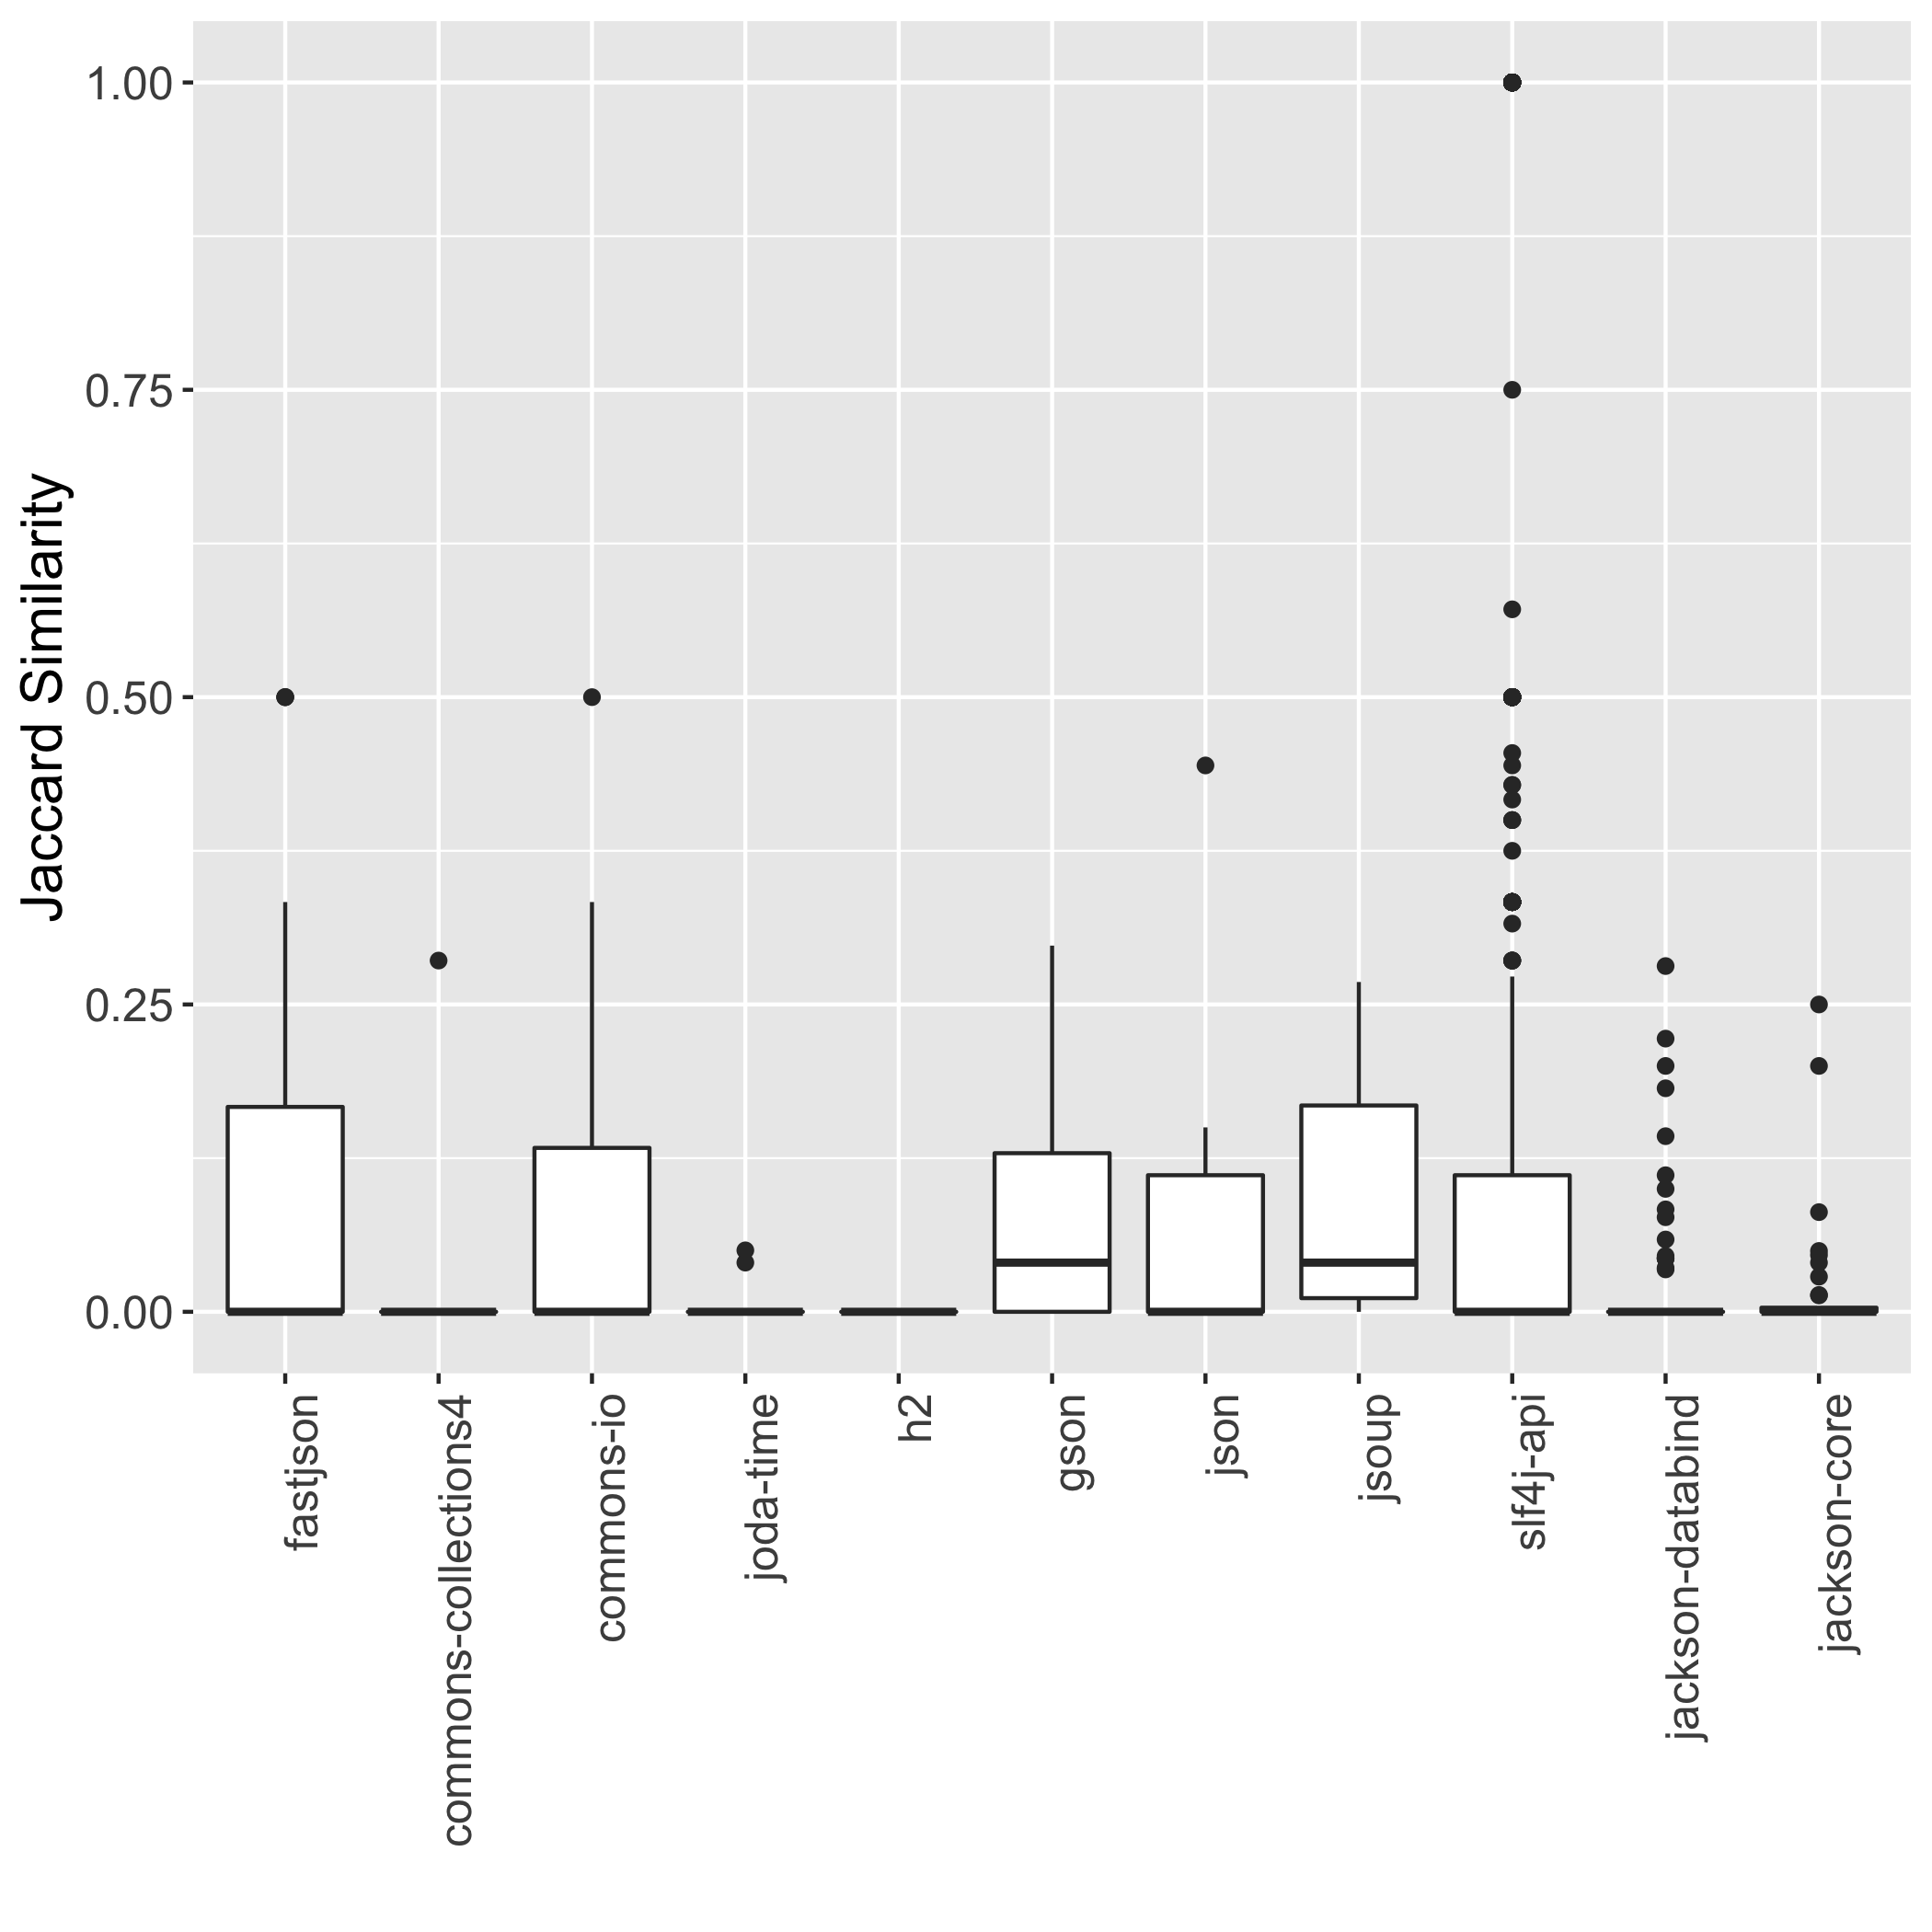
\includegraphics[width=8cm, height=7cm]{./images/jac-sim-box-plot-declared}
\caption{\label{fig:jaccard}Jaccard similarities between clients' API usages}
\end{figure}
\end{center}
%% Digging into \emph{fastjson}, we found that it is a ``mixed type'' library: some clients use APIs related
%% to \texttt{javax.ws.rs}, the JEE standard for restful services, while others use just a standalone parser API that does not implement an external specification. 


We were not surprised by the generally small amounts of overlap, because the libraries' exposed API surfaces tended
to have thousands of exposed elements and hundreds of used elements. Recall also our earlier discussion about \emph{fastjson} and how it could be fissioned into modules. Generally, across our benchmarks, small number of members are used by
multiple clients, but many others are used only once.

Table~\ref{tab:same-method} presents another view of API overlap between clients. We constructed the largest set
of methods shared by more than 1 client of a library (``max-set'') and report the size of that set as well as the percentage
of clients which use all of that set of methods. So, for \emph{gson}, we can see that there is one method shared
by all 4 clients, and no set of 2 methods shared by 2 clients. Interestingly, then, \emph{jackson-databind} has a core of 5
methods which are all used by 20\% (3) of its clients. We characterize the amount of overlap as generally low but not
nonexistent: a few methods are repeatedly used.

% latex table generated in R 4.2.0 by xtable 1.8-4 package
% Mon Aug 29 11:02:02 2022
\begin{table}[ht]
\centering
\begingroup\small
\begin{tabular}{l!{\color{verylightgray}\vrule}rrr}
Library & Total No.  & \% Clients calling  & No. of methods  \\ 
 & of clients & same methods & called by (\%) clients \\
   \arrayrulecolor{verylightgray}\hline
fastjson & 26 & 50 & 1 \\ 
  commons-collections4 & 6 & 50 & 1 \\ 
  commons-io & 9 & 44 & 1 \\ 
  joda-time & 9 & 56 & 1 \\ 
  h2 & 3 & 0 & 0 \\ 
  gson & 17 & 41 & 1 \\ 
  json & 4 & 75 & 1 \\ 
  jsoup & 4 & 75 & 10 \\ 
  slf4j-api & 89 & 51 & 2 \\ 
  jackson-databind & 23 & 26 & 1 \\ 
  jackson-core & 13 & 46 & 4 \\ 
\end{tabular}
\endgroup
\caption{\label{tab:same-method}\% of clients calling same methods} 
\end{table}


%{\bf Research Question 2.} (a) Do clients often use only a subset of the published API? How big is this subset? (b) For each library, is that subset consistent across clients? (c) Do different libraries show different usage patterns by clients?

\begin{mdframed}[
  leftmargin=\parindent,
  rightmargin=\parindent,
  skipabove=\topsep,
  skipbelow=\topsep
  ]
{\bf Finding 2:} APIs are sparsely used by clients---mostly methods (6\% utilization), but a few fields (3\%) and supertypes (6\%). There is limited but nonzero overlap between the methods used by different clients.
\end{mdframed}
